\documentclass[a4paper]{article}

\addtolength{\hoffset}{-2.25cm}
\addtolength{\textwidth}{4.5cm}
\addtolength{\voffset}{-3.25cm}
\addtolength{\textheight}{5cm}
\setlength{\parskip}{0pt}
\setlength{\parindent}{0in}

%----------------------------------------------------------------------------------------
%	PACKAGES AND OTHER DOCUMENT CONFIGURATIONS
%----------------------------------------------------------------------------------------

\usepackage{blindtext} % Package to generate dummy text
\usepackage{charter} % Use the Charter font
\usepackage[utf8]{inputenc} % Use UTF-8 encoding
\usepackage{microtype} % Slightly tweak font spacing for aesthetics
\usepackage[english]{babel} % Language hyphenation and typographical rules
\usepackage{amsthm, amsmath, amssymb} % Mathematical typesetting
\usepackage{float} % Improved interface for floating objects
\usepackage[final, colorlinks = true,
            linkcolor = black,
            citecolor = black]{hyperref} % For hyperlinks in the PDF
\usepackage{graphicx, multicol} % Enhanced support for graphics
\usepackage{xcolor} % Driver-independent color extensions
\usepackage{marvosym, wasysym} % More symbols
\usepackage{rotating} % Rotation tools
\usepackage{censor} % Facilities for controlling restricted text
\usepackage{listings} % Environment for non-formatted code, !uses style file!
\usepackage{pseudocode} % Environment for specifying algorithms in a natural way
 % Environment for f-structures, !uses style file!
\usepackage{booktabs} % Enhances quality of tables
\usepackage{tikz-qtree} % Easy tree drawing tool
 % Configuration for b-trees and b+-trees, !uses style file!
\usepackage[backend=bibtex,style=numeric,
            sorting=nyt]{biblatex} % Complete reimplementation of bibliographic facilities
\addbibresource{b.bib}
\usepackage{csquotes} % Context sensitive quotation facilities
\usepackage[yyyymmdd]{datetime} % Uses YEAR-MONTH-DAY format for dates
\renewcommand{\dateseparator}{-} % Sets dateseparator to '-'
\usepackage{fancyhdr} % Headers and footers
\pagestyle{fancy} % All pages have headers and footers
\fancyhead{}\renewcommand{\headrulewidth}{0pt} % Blank out the default header
\fancyfoot[L]{} % Custom footer text
\fancyfoot[C]{} % Custom footer text
\fancyfoot[R]{\thepage} % Custom footer text
\newcommand{\note}[1]{\marginpar{\scriptsize \textcolor{red}{#1}}} % Enables comments in red on margin
\usepackage{mathtools}
\usepackage{amsmath}
\DeclarePairedDelimiter\abs{\lvert}{\rvert}%
\usepackage{cancel}
\usepackage{minted}
\usepackage{float}
\usepackage{caption}
\usepackage{subcaption}
%-------------------------------

%----------------------------------------------------------------------------------------
\nocite{*}
%-------------------------------
%	ENVIRONMENT SECTION
%-------------------------------
\pagestyle{fancy}
\usepackage{mdframed}

\usepackage[sfdefault]{FiraSans} %% option 'sfdefault' activates Fira Sans as the default text font
\usepackage[T1]{fontenc}
\renewcommand*\oldstylenums[1]{{\firaoldstyle #1}}


% remove numbering from sections
\usepackage{titlesec}
\titleformat{\section}{\normalfont\Large\bfseries}{}{0pt}{}


% Reference


%-------------------------------------------------------------------------------------------
%	CUSTOM COMMANDS
%-------------------------------
\newcommand{\gaussian}{\frac{1}{\sigma\sqrt{2\pi}}\exp\left(- \frac{(x-\mu)^2}{2\sigma^2}\right)}
\newcommand{\R}{\mathbb R}
\newcommand{\norm}[1]{\lVert #1 \rVert}

\def\inline{\lstinline[basicstyle=\ttfamily,keywordstyle={}]}


\newcommand{\ps}{x^+}
\newcommand{\ns}{x^-}


\begin{document}


%-------------------------------
%	TITLE SECTION
%-------------------------------

\fancyhead[C]{}
\hrule \medskip % Upper rule
\begin{minipage}{0.295\textwidth}
  \raggedright
  \footnotesize
  Francisco Javier Sáez Maldonado \hfill\\
  franciscojavier.saez@estudiante.uam.es
  \hfill\\
\end{minipage}
\begin{minipage}{0.4\textwidth}
  \centering
  \large
  Speech Recognition using ESPNet\\

  \normalsize
  Deep Learning for Audio Signals\\
\end{minipage}
\begin{minipage}{0.295\textwidth}
  \raggedleft
  \today\hfill\\
\end{minipage}
\medskip\hrule

%-------------------------------
%	CONTENTS
%-------------------------------

\tableofcontents

\section*{Introduction}

In this assignment, we will present the Automatic Speech Recognition (ASR) task. The main goal of this task is to assign a sequence of words, letters or phonemes to a given input, which is usually audio features.

In particular, we will use an already \textbf{built} recognition system based in End-to-end deep learning. We will use \emph{ESPNet (End-to-end Speech Processing Toolkit)}. The code that we will use was provided by \href{https://scholar.google.com/citations?user=biA-c9sAAAAJ&hl=en}{Beltrán Labrador} and \href{https://scholar.google.es/citations?user=aENoFF4AAAAJ&hl=es}{Doroteo Torre}, and can be found in this \href{https://colab.research.google.com/drive/17JDlDB2ERa4YQAtKIaWfQysygPs7ao8W?usp=sharing}{Google Colab notebook}.

\section{Setting the environment up}

To test ESPNet, we will use the dataset \inline{TIMIT}, which contains \(6300\) phrases, divided in \(10\) phrases of each of the \(630\) speakers from the \(8\) main different US dialect regions. The phrases are also divided in male and female speakers. It is also important to remark that the division in train/test splits is done in a way that:
\begin{itemize}
  \item A speaker appears rather in the train or in the test split separately, but not in both at the same time.
  \item The phrases of the test set are \textbf{not} in the train set.
\end{itemize}

The first task will simply consists on looking at the content of the files that the \inline{TIMIT} corpus provides and understanding these files.\\

\textbf{Questions.}

\begin{itemize}
  \item \emph{Check the content of the .txt, .wrd and .phn files listening to the audio (.wav file) with a few examples. Comment how it was done and the results obtained.}\\

        To check the content of the files, we can use \inline{bash} commands. After loading the dataset in Google Colab, we store it in the \inline{content/timit/TIMIT} folder, in which we can find the \inline{TRAIN/TEST} folders. Having a look at the \href{https://catalog.ldc.upenn.edu/LDC93s1}{official documentation} and to the assignment documentation, we observe that we have the folders have the following structure:
        \begin{minted}{bash}
        <DIALECT>/<SEX><SPEAKER_ID>/<SENTENCE_ID>.<FILE_TYPE>
        \end{minted}

        We can list the different users of any of the regions and select one of them to observe his or her data. For convenience, we firstly use the code provided to examine the data of the user \inline{DR1/FCJF0}, meaning that it is an user from the first dialect region, and it is a female. We select the audio \inline{SX397} and then we show the \emph{spelling} of the phrase.

        \begin{minted}{bash}
          !cat /content/timit/TIMIT/TRAIN/DR1/FCJF0/SX397.TXT

          0 39220 Tim takes Sheila to see movies twice a week.
        \end{minted}

        We appreciate that this audio consist uniquely on one phrase. If we use
        \begin{minted}{Python}
           Ipython.display.audio('path_to_the_audio')
        \end{minted}
        (where the path in this case is\emph{/content/timit/TIMIT/TRAIN/DR1/FCJF0/SX397.WAV}), we listen to the audio and verify that the spelling is correct. We can also check the \emph{aligned word-level transcription}:

        \begin{minted}{bash}
          !cat /content/timit/TIMIT/TRAIN/DR1/FCJF0/SX397.WRD

            2240 5540 tim
            5540 8610 takes
            8610 14707 sheila
            14707 15791 to
            15791 19735 see
            19735 26402 movies
            26402 31210 twice
            31210 31791 a
            31791 37180 week
        \end{minted}
        Which indicates exactly the steps of time where the words happen, and we can lastly observe the phonetic transcription:

        \begin{minted}{bash}
          !cat /content/timit/TIMIT/TRAIN/DR1/FCJF0/SX397.PHN

          0 2240 h#
          2240 2940 t
          2940 4469 ih
          4469 5540 m
          5540 5860 tcl
          5860 6570 t
          6570 8211 ey
          8211 8610 kcl
          8610 11112 sh
          ...
        \end{minted}

        Since this is the provided example, we repeat the process with a different example to check that everything is correct in another case. We use the same region and female speaker. We select the sentence id: \inline{SX307}. We show the spelling transcription and the word-level transcription:

        \begin{minted}{bash}
          !cat /content/timit/TIMIT/TRAIN/DR1/FCJF0/SX307.TXT
          !echo "-----"
          !cat /content/timit/TIMIT/TRAIN/DR1/FCJF0/SX307.WRD

          0 23143 The meeting is now adjourned.
          -----
          1960 2616 the
          2616 8293 meeting
          8293 10160 is
          10960 13707 now
          13707 20887 adjourned
        \end{minted}

        Which shows the content of the phrase. Lastly, we have played the audio as we have explained before to check that the phrase is correct. We detect a little bit of noise on the speaker, but the words can be understood correctly.

  \item \emph{Explore the documentation of the TIMIT corpus and find information associated to the speakers. Can you think of any other applications of this corpus further from the training and evaluation of Speech Recognition systems?}\\


        We consider the folder structure mentioned before to give an answer to this. we find that we have audios classified by \emph{sex} and \emph{speaker}. Thanks to this, we could definitely use this corpus to build a \emph{male/female} recognition system or even a \textbf{speaker recognition system}. However, the available data for this kind of tasks would probably too low since this dataset is not focused on this task.

        Also, we know that we have both the \textbf{aligned word transcription} and the \textbf{aligned phonetic transcription} available, which could help us to create a \textbf{event detection system} with the capability of detecting the event: \emph{Speech}. However, it would be this unique event since it is the only one labeled in this dataset, so it would not be very useful, although this dataset could be joined with other events datasets to improve the event detection system.

        Lastly, in \href{https://catalog.ldc.upenn.edu/docs/LDC93S1/SPKRINFO.TXT}{this file of the documentation}, we observe that we can find more information about the speakers such as the race, birth date or education level. All this information could be use to perform different classification tasks, as we mentioned before with the sex. The birth date could be used for a regression problem using audio.
\end{itemize}

\section{ESPNet in Bash}

In this section, we will use ESPNet in \inline{Bash} to evaluate a STT system using end-to-end neural networks. We will use the previously presented corpus. The structure of stages that will have to be followed in order to train the system is presented in Figure \ref{fig:structure:stages}

\begin{figure}[H]
\centering
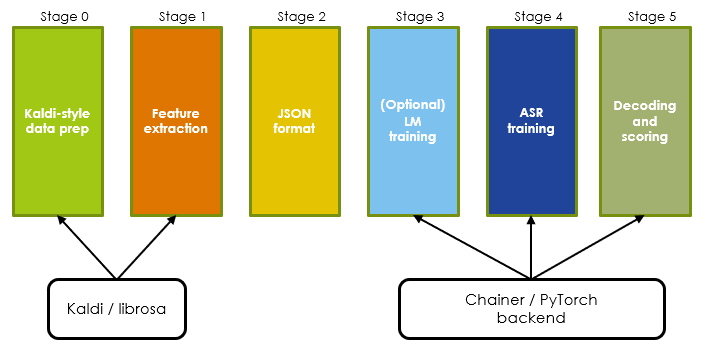
\includegraphics[scale=0.6]{Figures/stages}
\caption{Stages of the complete recipe.}
\label{fig:structure:stages}
\end{figure}

\subsection{Directory tree and KALDI recipes}

\begin{itemize}
  \item \emph{Which file(s) should be modified to change...:}\\
        \begin{itemize}
          \item The DNN backbone: The DNN backbone is specified in the file:
                \begin{minted}{bash}
      espnet/egs/timit/asr1/conf/train.yaml
    \end{minted}
                If we explore this file, we can see that we can specify the \emph{encoder} architecture, the \emph{decoder} architecture and also the attention related layers and hybrid CTC/attention parameters.
          \item The Seq-to-seq mapping used:
        \end{itemize}

  \item \emph{Comparing the obtained results in phoneme recognition and character recognition in the TIMIT corpus, which one do you consider more precise?}\\

        The results are shown in a \inline{Markdown} file. In this file, the number of files, words, the percentage of correct tokens, percentage of substitutions/deletions/insertions and the error rate are shown.

        For each of the cases (phoneme/character) a few different configurations of encoder, decoder and attention type are displayed. We resume the most most relevant information in Table \ref{table:results:1}.
        \begin{table}[H]
          \begin{tabular}{l|lllrr}
          Transcription type & Encoder        & Attention type              & Decoder       & \multicolumn{1}{l}{Accuracy on tokens} & \multicolumn{1}{l}{Error on tokens} \\ \hline
          Phonemes           & vggbgrup       & coverage\_location          & gru           & 82.1                                   & 21.4                                \\
                             & \textbf{bgrup} & \textbf{coverage\_location} & \textbf{lstm} & \textbf{82.7}                          & \textbf{20.2}                       \\
                             & bgrup          & location                    & gru           & 82.5                                   & 20.5                                \\
          Characters         & vggbgrup       & location                    & lstm          & 69.6                                   & 38.2                                \\
                             & vggbgrup       & location2d                  & gru           & 72.0                                   & 34.0                                \\
                             & bgrup          & coverage\_location          & lstm          & 72.8                                   & 33.7                               
          \end{tabular}
          \caption{Results on Phonemes and Characters recognition.}

          \label{table:results:1}
          \end{table}
          The results show that, in general, this system is \textbf{more capable of recognizing the phonemes} than the characters itself. There is a difference of about \(10\%\) in accuracy and more than \(15\%\) in the error rates. Recall that the error rates do not have to sum \(100\%\), since the error percentage can be higher than \(100\%\). In particular, in the shown cases, we obtain that the best performing system for phoneme recognition uses \inline{bgrup} as the encoder, an \inline{lstm} as decoder, and uses \inline{coverage_location} as the attention type, obtaining an accuracy of \(82.7\%\) on tokens and an error of \(20\%\).
\end{itemize}

\subsection{Data}
In this section we will prepare the data for the training of the system.

\textbf{Questions.}\\

\begin{itemize}
  \item \emph{What are the names of the three subsets of \inline{TIMIT} that are used? How many phrases does each of them have?}\\
  
  The subsets and the number of phrases are summarized in Table \ref{table:timit:subsets}.
  \begin{table}[H]
    \begin{tabular}{l|rrrr}
    Subset name & \multicolumn{1}{l}{Number of phrases} & \multicolumn{1}{l}{Mean duration} & \multicolumn{1}{l}{Min Duration} & \multicolumn{1}{l}{Max duration} \\ \hline
    train\_wav  & 3696                                  & 3.063                             & 0.915                            & 7.788                            \\
    dev\_wav    & 400                                   & 3.08                              & 1.09                             & 7.43                             \\
    test\_wav   & 192                                   & 3.03                              & 1.30                             & 6.21                            
    \end{tabular}
    \caption{Information about the used \inline{TIMIT} subsets.}
    \label{table:timit:subsets}
    \end{table}
  \item \emph{What are the "FBANK" features?}\\
  \textbf{FBANK} (Mel-filter bank coefficients) features are extracted from the raw audios. They can be compared with the known MFCCs(Mel Frequency Cepstral Coefficients), which are obtained using the FBANKS and the DCT. This is shown in \cite{FBANK}. The difference in the process can be observed in Figure \ref{fig:FBANKvsMFCC}.

  \begin{figure}[H]
    \centering
    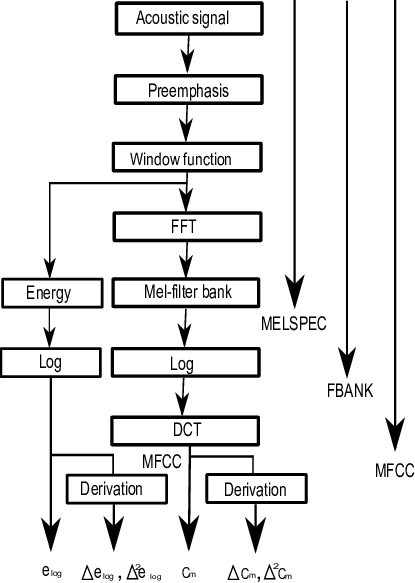
\includegraphics[scale=0.4]{Figures/FBANKvsMFCC.png}
    \caption{Obtention of FBANK and MFCCs.}
    \label{fig:FBANKvsMFCC}
  \end{figure}

  
  \item \emph{What does the acronym "CMVN" shown in the computational logs mean?}\\
  We have found in \href{https://en.wikipedia.org/wiki/Cepstral_mean_and_variance_normalization}{Wikipedia} that this acronym stands for \textbf{Cepstral Mean and Variance Normalization}, which is a computationally efficient normalization used in robust speech recognition.  This technique minimizes distortion by noise contamination, leading to \textbf{robust feature extraction}, linearly transforming the Cepstral coefficients.
\end{itemize}

\subsection{Training the neural networks.}

It is time to train the model and check its performance. 

\textbf{Questions.}\\

\emph{Examine the file} \inline{train.yalm} \emph{and try to identify which parameter should be modified in order to change:}
\begin{itemize}
  \item \emph{Number of encoder layers}: This is specified in the variable \inline{elayers}. 
  \item \emph{Encoder type}: This parameter is stored in the variable \inline{etype}
  \item \emph{Number of units per encoder layer}: It can be found in the variable \inline{eunits}.
  \item \emph{Encoder attention type}: The variable \inline{atype} indicates this.
  \item \emph{Number of units in encoder}: This is stored in the variable \inline{dunits}.

\end{itemize}
The variable names are self-explicative and the file \inline{train.yalm} is properly commented so finding the answers was easy. Usually, variables related to the encoder start with \inline{e}, the attention variables start with \inline{a} and the decoder variables begin with \inline{d}, making the script intuitive.\\

\textbf{Tensorboard} can be used to graphically analyze the evolution of the training.\\

\textbf{Question.}
\begin{itemize}
\item \emph{Can you identify the parameters that correspond to the CTC (Connectionst temporal classification) and attention?}
\item \emph{Check the evolution of the different parameters and the evolution in train and validation. Do you consider that the training has worked correctly? }
\end{itemize}

\emph{ESPNet} also generates charts about the trainig process.\\

\textbf{Questions.}
\begin{itemize}
\item \emph{Can you observe any difference between the evolutions associated to CTC and attention? Why?}
\item \emph{What is the final approximated PER in train and validation? Why are the results different? }
\end{itemize}

\subsection{Recognition and evaluation}

In this section, we will examine the file \inline{decode.yalm} and answer some questions about it.

\textbf{Questions.}
\begin{itemize}
\item \emph{What does the parameter} \inline{beam-size} \emph{do?}\\

The parameter \inline{beam-size} controls the number of hypotheses kept during the Beam Search (found in the \href{https://espnet.github.io/espnet/_gen/espnet.nets.html?highlight=beam#espnet-nets-batch-beam-search}{documentation} of the \inline{beam search} implementation).

As a note for myself, \textbf{beam search} is
\item \emph{What does the parameter} \inline{ctc-weight} \emph{do?}\\
\end{itemize}


\printbibliography
\end{document}
